% \documentclass[8pt,xcolor=pdftex,table,handout]{beamer}

\documentclass[8pt,xcolor=pdftex,table]{beamer}
\mode<presentation>

\usepackage[utf8]{inputenc}
\usepackage{lmodern}
\usepackage[T1]{fontenc}


% \usepackage{mathenv}
\usepackage{array}
% \usepackage{amsmath}
\usepackage{mathtools}% Loads amsmath
\usepackage{wasysym}
\usepackage{amsfonts}
\usepackage{amssymb, amsbsy}
\usepackage[utf8]{inputenc}
\usepackage{graphicx}
\usepackage{multimedia}
\usepackage{multicol}
\usepackage{multirow}
\usepackage{fourier}
\usepackage{makecell}


% \usepackage{colortbl}

% %\usepackage{textcomp}
% \usepackage{eurosym}

% % \usepackage{color}

% \usepackage{cancel}
% \usepackage{enumitem}

%\usepackage[active,tightpage]{preview}
% \usepackage{times}
\usepackage{tikz}
\usetikzlibrary{shapes,arrows,shadows,calc, angles}
\usetikzlibrary{arrows,shapes}
\usetikzlibrary{positioning}

\usepackage{verbatim}

\tikzstyle{format} = [draw, thin, fill=blue!20]
\tikzstyle{medium} = [ellipse, draw, thin, fill=green!20, minimum height=2.5em]


\tikzstyle{box_style0}=[draw, rounded corners ,
anchor=center,text centered,text=white, font=\bfseries] % text width=33mm,

\tikzstyle{box_style}=[box_style0, fill=black!80] % text width=33mm,

% \tikzstyle{bStyle}=[draw, rounded corners , fill=black!80,
% anchor=base, text centered,text=white, text width=2.8cm,font = 33]
\tikzstyle{bStyle2}=[draw, rounded corners , fill=black!80,
anchor=base,text centered,text=white, font=\bfseries] % text width=33mm,

\tikzstyle{bStyle0}=[draw, rounded corners , fill=b1,
anchor=base,text centered,text=white, font=\bfseries, align=center] % text width=33mm,
\tikzstyle{bStyle1}=[draw, rounded corners , fill=g1,
anchor=base,text centered,text=white, font=\bfseries] % text width=33mm,

\tikzstyle{bStyle3}=[draw, rounded corners , fill=r1,
anchor=base,text centered,text=white, font=\bfseries, align=center] % text width=33mm,

\tikzstyle{myarrow0}=[->, >=triangle 60, very thick, rounded corners=1mm]
\tikzstyle{myarrow}=[->, >=stealth, very thick, rounded corners=2mm]
\tikzstyle{line}=[thick]


% \usepackage[final]{movie15}
% \usepackage{media9}

%\setbeamertemplate{mini frame in other subsection}[default][0]

% \usepackage{ulem}

% \usepackage{stackengine}
\usepackage[cm]{sfmath}
\renewcommand\dot[1]{\text{\stackon[1pt]{$#1$}{.}}}

% \usepackage{siunitx}
% \sisetup{detect-all}   % ...this to force siunitx to actually use your fonts
% \usepackage{helvet}    % set the normal font here
% \usepackage{sansmath}  % load up the sansmath so that math -> helvet
% \sansmath               % <- tricky! -- gotta actually tell tex to use!


\beamertemplatenavigationsymbolsempty

\newcommand{\RightCrlBrc}[1]{$\pmb{\left. \rule{0pt}{#1}\right\}} $}

\newcommand{\TextSoulign}[3]{\textcolor{#1}{\underline{#2\textcolor{black}{#3}}}}
\newcommand\dgs[0]{$^\circ$}
\newcommand\dgsC[0]{$\,^{\circ}{\rm C}$}

\newcommand\up[1]{$^{\text{#1}}$}
\newcommand*\dif{\mathop{}\!\textnormal{\slshape d}}


\newcommand\tbf[1]{\textbf{#1}}
\newcommand\tit[1]{\textit{#1}}
\newcommand\tcit[2]{\textcolor{#1}{\textit{#2}}}

\newcommand{\chckmrk}[0]{\Large \textcolor{mygreen}{\checkmark}}

\definecolor{myOrng}{rgb}{0.9,0.5,0}
\renewcommand{\alert}[1]{\textcolor{myOrng}{\tbf{#1}}}




\PassOptionsToPackage{unicode}{hyperref}
\PassOptionsToPackage{naturalnames}{hyperref}

\usetheme[titleformat=smallcaps, subsectionpage=progressbar]{metropolis} % usetitleprogressbar, subsectionpage=progressbar
% default, professionalfonts, serif, structurebold, structureitalicserif, structuresmallcapsserif
% \usefonttheme{professionalfonts}

% \usetikzlibrary{calc,decorations.pathmorphing,decorations.pathreplacing}
% \usetikzlibrary{calc,trees,positioning,arrows,chains,shapes.geometric,%
%     decorations.pathreplacing,decorations.pathmorphing,shapes,%
%     matrix,shapes.symbols}
%     \usepackage{tikz-3dplot}
% \usetikzlibrary{patterns}


% \usetheme[compress]{Berlin}
\definecolor{g1}{rgb}{0,0.4,0}
\definecolor{b1}{rgb}{0,0,0.6}
\definecolor{r1}{rgb}{0.7,0,0}
\definecolor{k1}{rgb}{0.2,0.2,0.2}



\definecolor{myBckgrd}{rgb}{0,0,0}
\definecolor{myShaded}{rgb}{0.5,0.5,0.5}
\definecolor{myFnt}{rgb}{0.84,0.84,0.84}

\definecolor{clrBorders}{rgb}{0,0,0}
% \definecolor{clrBorders}{rgb}{1,1,1}

\definecolor{violetOC}{rgb}{0.455,0.318,0.922}

\definecolor{dfFirstRow}{rgb}{0.18,0.18,0.18}
\definecolor{dfEvenRow}{rgb}{0.118,0.118,0.118}
\definecolor{dfOddRow}{rgb}{0.149,0.149,0.149}




\definecolor{myCyan}{rgb}{0,0.8,0.99}
\definecolor{mygreen}{rgb}{0,0.35,0}
\definecolor{myGreen}{rgb}{0,0.8,0}
\definecolor{myred1}{rgb}{0.2,0,0}
\definecolor{myred2}{rgb}{0.4,0,0}
\definecolor{myred3}{rgb}{0.6,0,0}

% \setbeamercolor*{background}{c3}
% \setbeamercolor*{palette primary}{use=structure,fg=white,bg=myred3}
% \setbeamercolor*{palette secondary}{use=structure,fg=white,bg=myred2}
% \setbeamercolor*{palette tertiary}{use=structure,fg=white,bg=myred1}
% \setbeamercolor*{palette quaternary}{use=structure,fg=white,bg=myred1}
% \setbeamercolor{father}{fg=red}
% \setbeamercolor{mother}{fg=black}
% %\setbeamercolor{child}{parent={father,mother}}
% % \setbeamercolor{enumerate item}{parent=item} \setbeamercolor{enumerate subitem}{parent=subitem} \setbeamercolor{enumerate subsubitem}{parent=subsubitem}
% \setbeamercolor{item}{use={father,mother text},fg=father.fg!55!mother text.fg}





\setbeamercolor{button}{bg=myred3,fg=black}


% \author[Durand-Texte]{Thomas Durand-Texte - thomas.durand-texte@univ-lemans.fr}}


%\pgfdeclareimage[height=0,25cm]{logoCNAM}{/users/LABO/recherche/Completion/figures/Logo_cnam.jpg}
%\pgfdeclareimage[height=0,25cm]{logoCNAM}{Logo_cnam}
%\logo{\pgfuseimage{logoCNAM}}
\linespread{1.4}


% background image
% \pgfdeclareimage[height=96mm,width=128mm]{nombidon}{ploum}
% \setbeamertemplate{background}{\pgfuseimage{nombidon}}




\setbeamertemplate{footline}[frame number]



\makeatletter
\let\beamer@writeslidentry@miniframeson=\beamer@writeslidentry
\def\beamer@writeslidentry@miniframesoff{%
	\expandafter\beamer@ifempty\expandafter{\beamer@framestartpage}{}% does not happen normally
	{%else
		% removed \addtocontents commands
		\clearpage\beamer@notesactions%
	}
}
\newcommand*{\miniframeson}{\let\beamer@writeslidentry=\beamer@writeslidentry@miniframeson}
\newcommand*{\miniframesoff}{\let\beamer@writeslidentry=\beamer@writeslidentry@miniframesoff}
\makeatother

\defbeamertemplate*{headline}{miniframes theme no subsection}
{%
	\begin{beamercolorbox}[colsep=1.5pt]{upper separation line head}
	\end{beamercolorbox}
	% \begin{beamercolorbox}{section in head/foot}
	% 	\vskip2pt\insertnavigation{\paperwidth}\vskip2pt
	% \end{beamercolorbox}%
	% \begin{beamercolorbox}[colsep=1.5pt]{lower separation line head}
	% \end{beamercolorbox}
}

\setbeamertemplate{footline}[miniframes theme no subsection]

\setbeamerfont{subsubsection in toc}{size=\normalsize}
\setbeamercolor{section in toc}{fg=black}
\setbeamercolor{subsection in toc}{fg=black}

\makeatletter
\setbeamertemplate{footline}{%
	\begin{beamercolorbox}[colsep=1.5pt]{upper separation line foot}
	\end{beamercolorbox}
	% \begin{beamercolorbox}[ht=2.5ex,dp=1.125ex,%
	% 	leftskip=.3cm,rightskip=.3cm plus1fil]{author in head/foot}%
	% 	\leavevmode{\usebeamerfont{author in head/foot}\insertshortauthor}%
	% 	\hfill%
	% 	{\usebeamerfont{institute in head/foot}\usebeamercolor[fg]{institute in head/foot}\insertshortinstitute}%
	% \end{beamercolorbox}%
	\begin{beamercolorbox}[ht=2.5ex,dp=1.125ex,%
		leftskip=.3cm,rightskip=.3cm plus1fil]{title in head/foot}%
		{\usebeamerfont{title in head/foot}\insertshorttitle\hfill\insertframenumber}%
	\end{beamercolorbox}%
	\begin{beamercolorbox}[colsep=1.5pt]{lower separation line foot}
	\end{beamercolorbox}
}
\makeatletter


% \tiny
% \scriptsize
% \footnotesize
% \small
% \normalsize
% \large
% \Large
% \LARGE
% \huge
% \Huge




%
% \definecolor{myBckGrd}{rgb}{0.9,0.9,0.9}



% \setbeamercolor{palette quaternary}{bg=black,fg=white}

% \setbeamercolor{background canvas}{bg=black}
% \color{white}


\newcommand\bsqr{\rule{0.7ex}{0.7ex}\hspace{0.74mm}}



\newcommand\shdd[1]{\textcolor{myShaded}{#1}}
\newcommand\shdng[4]{\only<#1>{\textcolor{myBckgrd}{#4}}%
									\only<#2>{#4}%
									% #3}
									\only<#3>{\shdd{#4}}}

\newcommand\clrItmz[1]{\setbeamercolor{itemize/enumerate body}{fg=#1} \setbeamercolor{item}{fg=#1}}
\newcommand\shdItmz[0]{\clrItmz{myShaded}}


\setbeamercolor{palette primary}{bg=myBckgrd,fg=black!60}
\setbeamercolor{normal text}{fg=myFnt,bg=myBckgrd}
\setbeamercolor{structure}{fg=white}

\newcommand\Wider[2][3em]{%
\makebox[\linewidth][c]{%
  \begin{minipage}{\dimexpr\textwidth+#1\relax}
  \raggedright#2
  \end{minipage}%
  }%
}

\setbeamerfont{frametitle}{size=\small}


\usepackage{listings}


% \usepackage{amsmath}
% \usepackage{unicode-math}
% \setmathfont{Fira Math}


\usepackage{animate}

% ------------------------------------------- %

\graphicspath{{Figures/} {Figures/Logos/}}
% \graphicspath{{../Figures/} {../Figures/Logos/}}

\title[]{\vspace{22mm}Formation Ingénieur Machine Learning\\\vspace{6mm}Projet: Définissez votre stratégie d'apprentissage}
\date[]{5 Janvier 2023\\\vspace{18mm}\\\tit{thomas.durandtexte@protonmail.com}}


\titlegraphic{\hfill
\def\arraystretch{.1}%  1 is the default, change whatever you need
	\begin{tabular}{ >{\centering}m{7mm} m{39mm} }
		
\includegraphics[height=7mm]{Logo_OpenClassrooms.png }
		&
		\Large{\textbf{OPENCLASSROOMS}}
	\end{tabular}
	
	% \begin{tabular}{ >{\centering}m{26mm} >{\centering}m{36mm} >{\centering}m{10mm} >{\centering}m{20mm} }
	% 	% \includegraphics[height=10mm]{FullFields_Logo.png}
		
	% 	}
	% 	&
	% 	\includegraphics[height=8.8mm]{1280px-Logo_Univ_du_Maine.png} &
	% 	\includegraphics[height=10mm]{logoCNRS.png} &
	% 	\includegraphics[height=16mm]{LAUM_white.png}
	% \end{tabular}
	% 	% \includegraphics[height=10mm]{FullFields_Logo.png} \hspace{2mm}
	% 	% \includegraphics[height=8.8mm]{1280px-Logo_Univ_du_Maine.png} \hspace{2mm}
	% 	% \includegraphics[height=10mm]{logoCNRS.png} \hspace{2mm}
	% 	% \includegraphics[height=13mm]{LAUM.png}
}



\begin{document}
% ------------------------------------------- %

\begin{frame}
	\titlepage

	% \vspace{-6mm}
	% \begin{center}
	% 	\begin{tabular}{>{\centering}m{20mm}>{\centering}m{12mm}>{\centering}m{24mm}>{\centering}m{30mm}}
	% 		\includegraphics[width=20mm]{LogoInst_LAUM.png} &
	% 		\includegraphics[height=10mm]{logoCNRS.jpeg} &
	% 		\includegraphics[height=6mm]{1280px-Logo_Univ_du_Maine.png} &
	% 		\includegraphics[height=10mm]{FullFields_Logo+baseline2.png}
	% 	\end{tabular}
	% \end{center}
\end{frame}




% ------------------------------------------- %
% \begin{frame}[standout]
% 	Studied object:\\
% 	\alert{Clamped} - \alert{Free} ceramic
% \end{frame}
% ------------------------------------------- %


% ------------------------------------------- %
\section{Mon parcours}


% \subsection{Simulations}


\begin{frame}[t]
	\vspace{3mm}
	\shdd{Parcours}
	
	\begin{center}
		
		\begin{tikzpicture}
			\node[box_style] (Inge) at (0,0) {{Diplôme ingénieur}} ;
			\node[box_style] (IMDEA) at (40mm,0) {Master internationnal} ;
			\draw[myarrow] (Inge.north) to [out=50, in=130] (IMDEA.north) ;
			\node[box_style] (phd) at (20mm,-28mm) {Thèse} ;
			\draw[myarrow] (IMDEA.south) to [out=-80, in=90] (phd.north) ;
			\node[box_style, text width=21mm] (postdoc) at (20mm,-40mm) {{4 ans recherche\\\vspace{-1mm}post-doctorale}} ;
			\draw[myarrow] (phd.south) -- (postdoc.north) ;
			
			\node (OC) at (20mm,-55mm) {
\includegraphics[width=8mm]{Logo_OpenClassrooms.png}} ;

			\node at (-20mm,-30mm) {
				\movie[height=50mm]{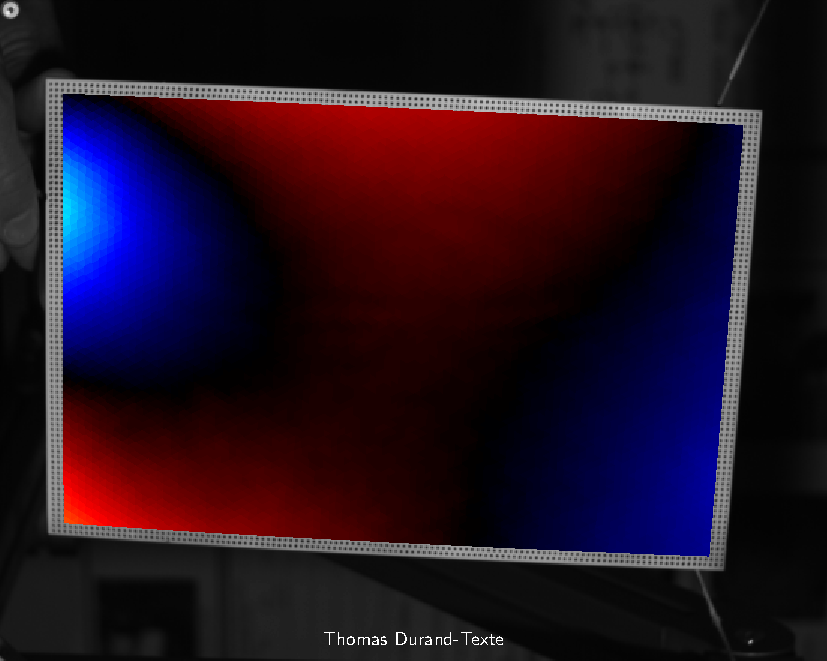
\includegraphics[width=50mm, angle=90]{Plate/Movie_plate.pdf}}{Movie_plate.mp4}
			};
		\end{tikzpicture}
	\end{center}
\end{frame}
	

\begin{frame}
	\begin{overlayarea}{\textwidth}{\textheight}

		\vspace{6mm}
	\shdd{Parcours}
	\begin{itemize}
		\item[\shdng{0}{1}{2-}{$\bullet$}] \shdng{0}{1}{2-}{Ingénieur spécialisé Vibro-acoustique}
		\item[\shdng{-1}{2}{3-}{$\bullet$}] \shdng{-1}{2}{3-}{Master internationnal en Électro-Acoustique}
		\item[\shdng{-2}{3-7}{8-}{$\bullet$}] \shdng{-2}{3-7}{8-}{Doctorat : mesure de vibrations par vision 3D}
		\item<8->[\shdng{-7}{8-}{0}{$\bullet$}] Recherche post-doctoral (4 ans) :
		\only<9->{
		\begin{itemize}
			\item[$\bullet$] Imagerie infra-rouge appliqué à la dissipation vibratoire
			\item[$\bullet$] Création de modèles : mécanique \& thermique (et couplage des 2)
			\item[$\bullet$] Étude de vibrations de céramiques
		\end{itemize}}
		\item<10>[$\bullet$] Recherche personnelle ?
	\end{itemize}

	\only<1>{
		\vspace*{-30mm}
		\hspace*{60mm}
		\movie[loop,width=40mm]{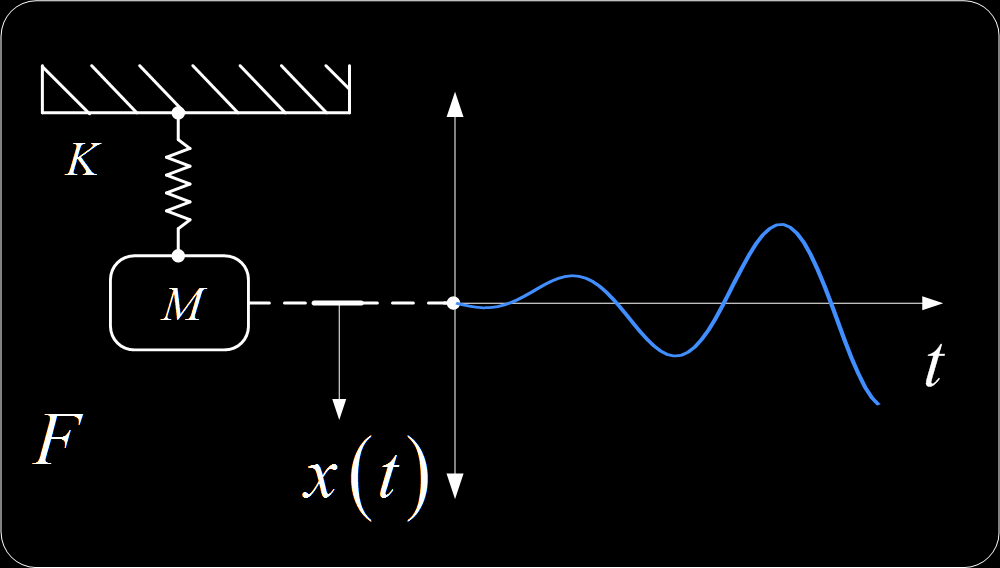
\includegraphics[width=40mm]{vib/Mass_Spring_dark-0.png}}{mass_spring.mp4}
	}

	\only<2>{
		\vspace*{-25mm}
		\hspace*{70mm}
		
\includegraphics[width=20mm]{electroac/loudspeaker.pdf}
	}

	\vspace{3mm}
	\only<-3>{
		\visible<3>{
			\centering
			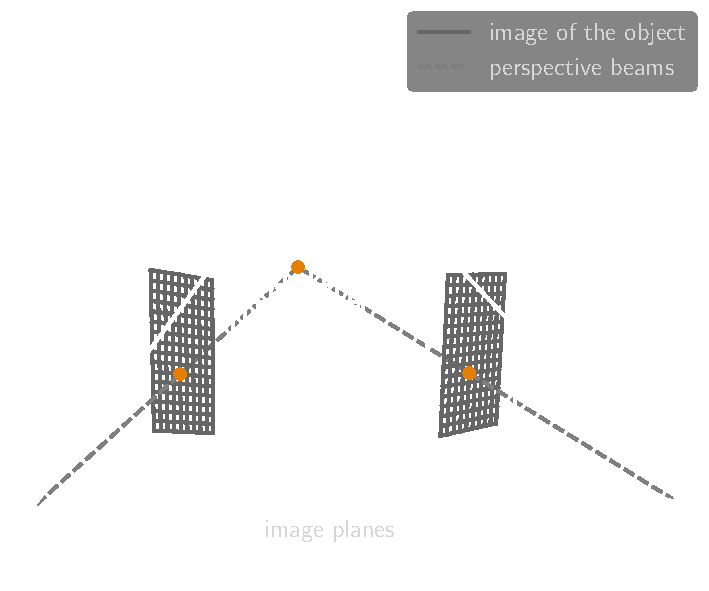
\includegraphics[width=70mm]{triangulation.pdf}
		}
	}
	\only<4>{
	\begin{figure}
		\centering
		\movie[width=70mm]{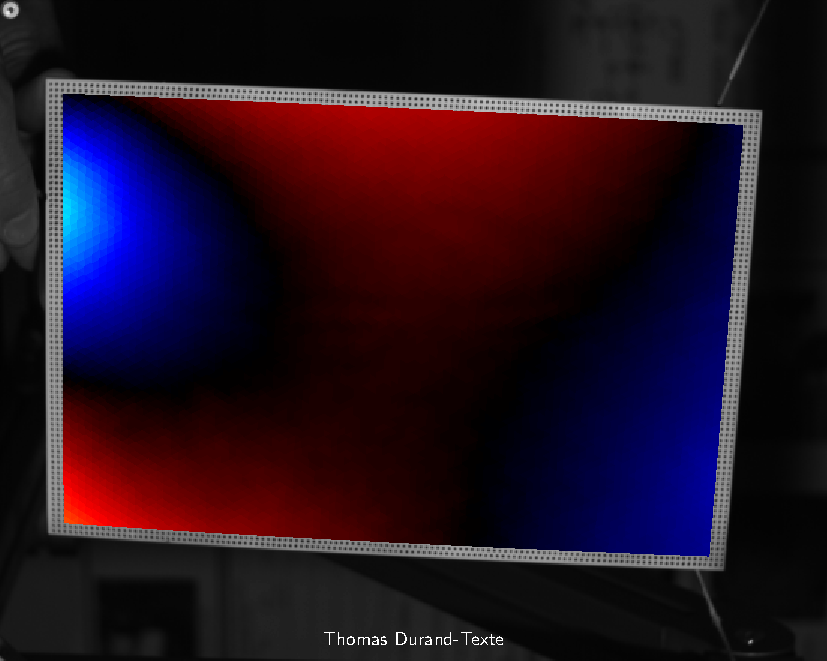
\includegraphics[width=70mm]{Plate/Movie_plate.pdf}}{Movie_plate.mp4}
	\end{figure}
    }
	\only<5>{
		\centering
		\shdd{Estimation pour 1 point}\\
		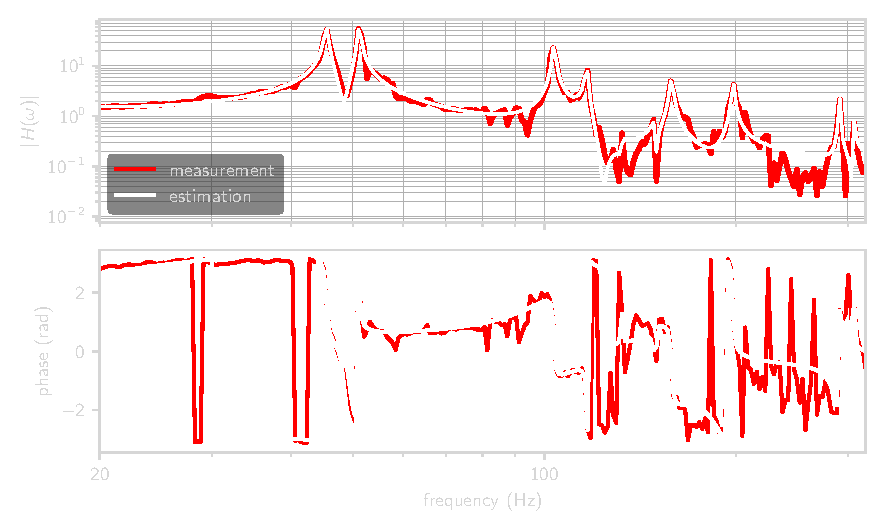
\includegraphics[width=80mm]{Plate/estimated_FRF.pdf}
	}
	\only<6-7>{
		\centering
		\shdd{Estimation par mode}
		\begin{tabular}{cc}
			\only<6>{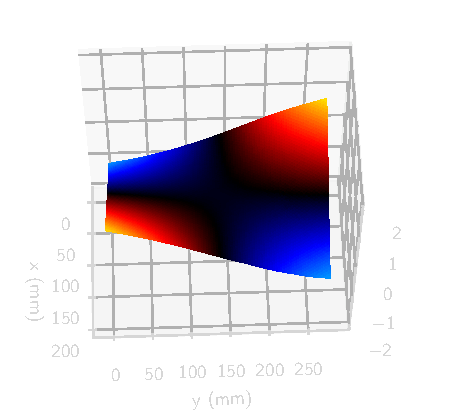
\includegraphics[width=60mm]{Plate/DS_n/1.pdf}}%
			\only<7>{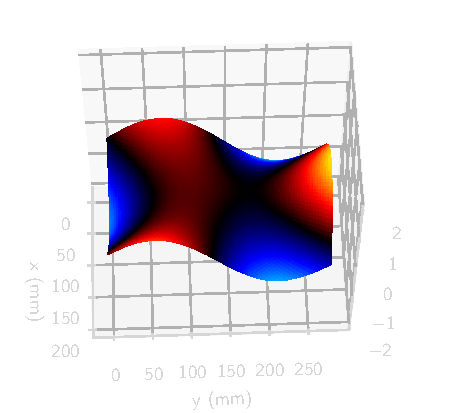
\includegraphics[width=60mm]{Plate/DS_n/5.pdf}}%
			&
			\only<6>{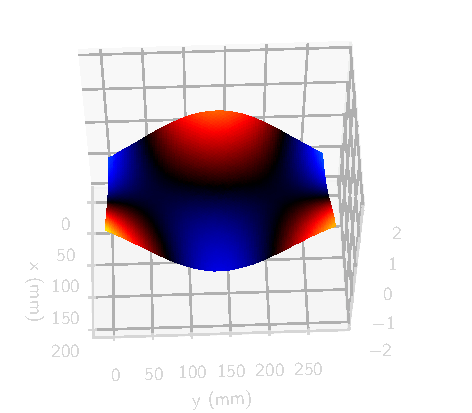
\includegraphics[width=60mm]{Plate/DS_n/3.pdf}}%
			\only<7>{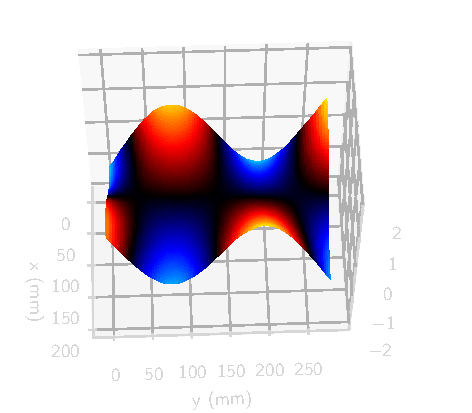
\includegraphics[width=60mm]{Plate/DS_n/8.pdf}}%
		\end{tabular}
	}

	\end{overlayarea}
\end{frame}

\section{Pourquoi une nouvelle formation ?}

\begin{frame}[t]
	\vspace{6mm}
	\shdd{Une nouvelle formation pour :}
	\begin{itemize}
		\item[\shdng{0}{1}{2-}{$\bullet$}] \shdng{0}{1}{2-}{Le plaisir d'apprendre}
		\item[\shdng{-1}{2}{3-}{$\bullet$}] \shdng{-1}{2}{3-}{Élargir mon champs de compétence}
		\item[\shdng{-2}{3}{4-}{$\bullet$}] \shdng{-2}{3}{4-}{Pouvoir accéder à plus d'applications}
	\end{itemize}

	\vspace*{-25mm}
	\hspace*{50mm}
	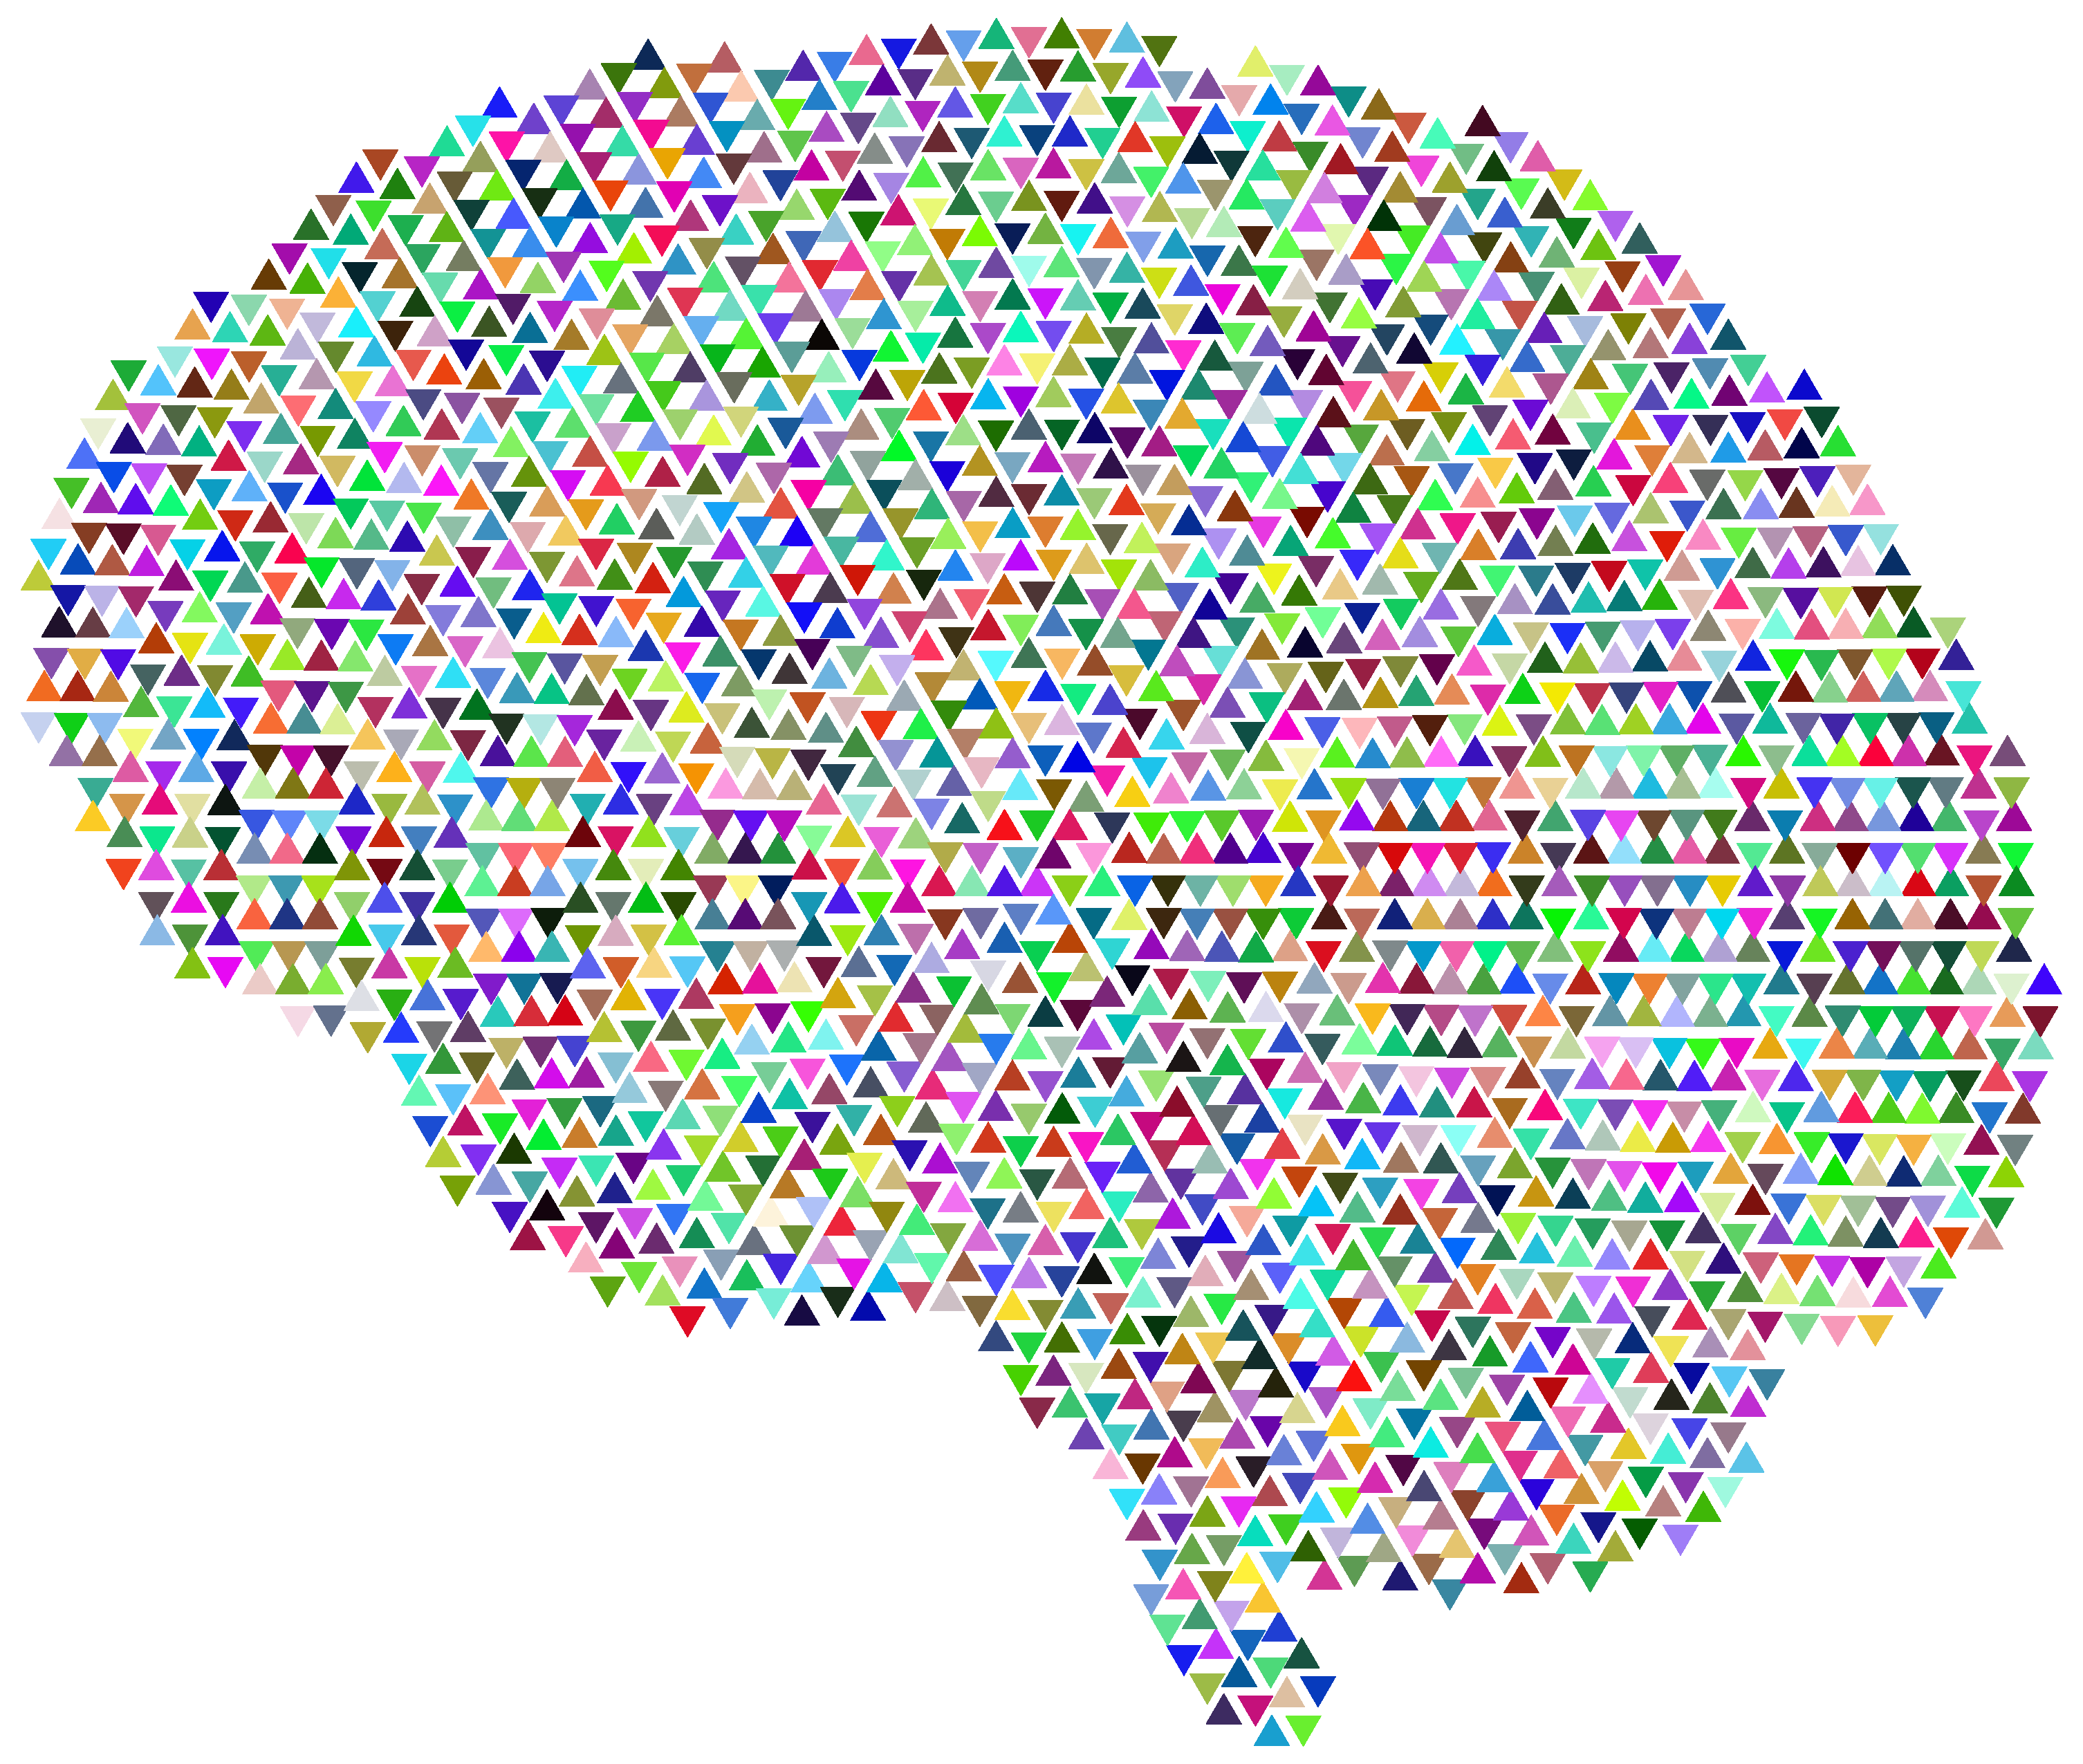
\includegraphics[width=20mm]{divers/brain.pdf}

		\visible<2->{
	\vspace*{-8mm}
	\hspace*{70mm}
	
\includegraphics[width=20mm]{divers/Prismatic-Cloud-Gears-2.pdf}
	}

	\vspace{7mm}
	\visible<4>{
	Objectif après la formation :\\
	\begin{center}
		\Huge Créer une micro-entreprise (freelance)
	\end{center}
	}
	\vspace{7mm}
\end{frame}


\section{Pourquoi OpenClassrooms ?}

\begin{frame}[t]
	\vspace{18mm}

	\shdd{Une formation OpenClassrooms c'est :}
	\begin{itemize}
		\item[\shdng{0}{1}{2-}{$\bullet$}] \shdng{0}{1}{2-}{45 minutes / semaine de mentorat avec un professionnel}
		\item[\shdng{-1}{2}{3-}{$\bullet$}] \shdng{-1}{2}{3-}{En distanciel (souplesse)}
		\item[\shdng{-2}{3}{4-}{$\bullet$}] \shdng{-2}{3}{4-}{Un accès à une communauté}
		\item[\shdng{-3}{4}{0}{$\bullet$}] \shdng{-3}{4}{0}{Un apprentissage par \only<4>{\alert{projets}}}
	\end{itemize}

	\visible<2->{
		\vspace*{-18mm}
		\hspace*{77mm}
		
\includegraphics[width=20mm]{divers/icon-computer.pdf}
	}

	\visible<3->{
	\vspace*{-12mm}
	\hspace*{45mm}
	\begin{tikzpicture}
		\only<3>{\node {
\includegraphics[width=20mm]{Slack_logo_white.pdf}} ; }
        \only<4->{\node[opacity=0.5] {
\includegraphics[width=20mm]{Slack_logo_white.pdf}};}%
    \end{tikzpicture}
	}

	\vspace{3mm}
	\begin{center}
		\only<4>{\hspace{0mm} 
\includegraphics[width=25mm]{divers/project-time.pdf}}
	\end{center}

	
	
\end{frame}




\section{Les projets}

\begin{frame}
	\shdd{Les projets :}
	\begin{itemize}
		\item[\shdng{0}{1}{2-}{1.}] \shdng{0}{1}{2-}{Concevez une application au service de la santé publique\newline(Gestion de données incomplètes)}
		\item[\shdng{-1}{2}{3-}{2.}] \shdng{-1}{2}{3-}{Anticipez les besoins en consommation de bâtiments\newline(Modèle d'apprentissage supervisé)}
		\item[\shdng{-2}{3}{4-}{3.}] \shdng{-2}{3}{4-}{Segmentez des clients d'un site e-commerce\newline(Modèle d'apprentissage non supervisé)}
		\item[\shdng{-3}{4}{5-}{4.}] \shdng{-3}{4}{5-}{Catégorisez automatiquement des questions\newline(Gestion de données non structurées \& extraction de features)}
		\item[\shdng{-4}{5}{6-}{5.}] \shdng{-4}{5}{6-}{Classez des images à l'aide d'algorithmes de Deep Learning\newline(Gestion d'images \& Deep Learning)}
		\item[\shdng{-5}{6}{7-}{6.}] \shdng{-5}{6}{7-}{Développez une preuve de concept\newline(Veille technologique \& preuve de concept)}
		\item[\shdng{-6}{7}{0}{7.}] \shdng{-6}{7}{0}{Participez à une compétition Kaggle !\newline(Mise en pratique, gestion \& communication de projet de développement)}
	\end{itemize}
\end{frame}

\begin{frame}
	\shdd{Les projets  les plus \alert{motivants} :}
	
	\vspace{6mm}
	\def\arraystretch{2}%  1 is the default, change whatever you need
	\begin{tabular}{>{\centering}m{50mm}c>{\centering}m{40mm}}
		\shdng{0}{1}{2-}{Concevez une application au service de la santé publique}
		&
		\shdng{0}{1}{2-}{\Huge $\rightarrow$}
		&
		\shdng{0}{1}{2-}{alimentation, prie en main des outils}
		\tabularnewline
		\shdng{-1}{2}{3-}{Anticipez les besoins en consommation de bâtiments}
		&
		\shdng{-1}{2}{3-}{\Huge $\rightarrow$}
		&
		\shdng{-1}{2}{3-}{modélisation, énergie}
		\tabularnewline
		\shdng{-2}{3}{0}{Classez des images à l'aide d'algorithmes de Deep Learning}
		&
		\shdng{-2}{3}{0}{\Huge $\rightarrow$}
		&
		\shdng{-2}{3}{0}{traitement d'images, (Deep learning?)}
	\end{tabular}
\end{frame}


\begin{frame}
	\shdd{Les projets  les plus \alert{difficiles} à priori :}
	
	\vspace{6mm}
	\def\arraystretch{2}%  1 is the default, change whatever you need
	\begin{tabular}{>{\centering}m{50mm}c>{\centering}m{40mm}}
		\shdng{0}{1}{2-}{Segmentez des clients d'un site e-commerce}
		&
		\shdng{0}{1}{2-}{\Huge $\rightarrow$}
		&
		\shdng{0}{1}{2-}{plus éloigné de mes compétences}
		\tabularnewline
		\shdng{-1}{2}{3-}{Catégorisez automatiquement des questions}
		&
		\shdng{-1}{2}{3-}{\Huge $\rightarrow$}
		&
		\shdng{-1}{2}{3-}{plus éloigné de mes compétences}
		\tabularnewline
		\shdng{-2}{3}{0}{Participez à une compétition Kaggle !}
		&
		\shdng{-2}{3}{0}{\Huge $\rightarrow$}
		&
		\shdng{-2}{3}{0}{compétition}
	\end{tabular}
\end{frame}


\begin{frame}[t]
	\vspace{3mm}
	\shdd{Dates prévisionnelles de soutenances :}

	\vfill
	\only<1>{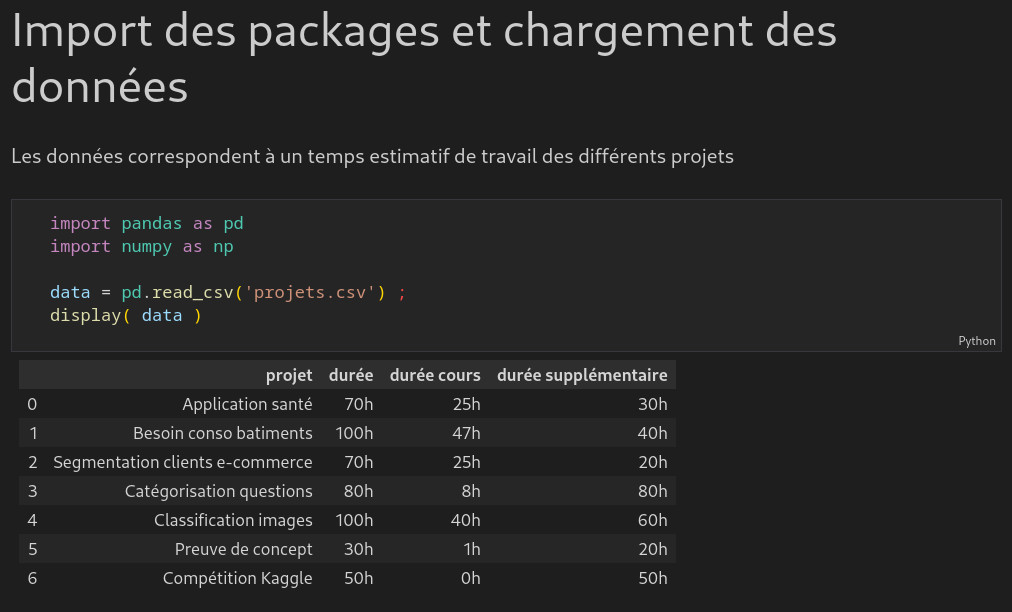
\includegraphics[width=110mm]{dates/cell-1.jpg}}%
	% \only<2>{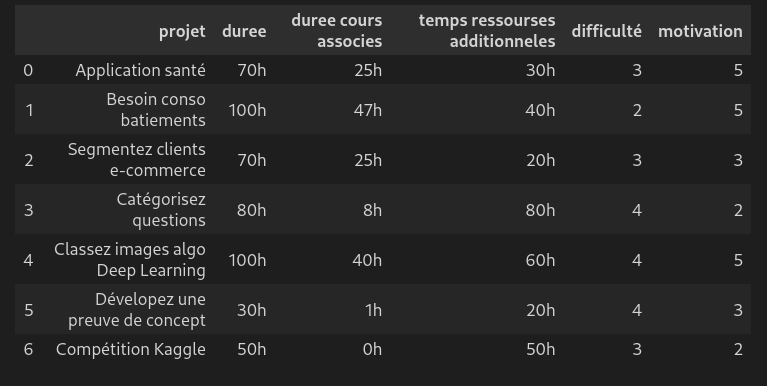
\includegraphics[width=110mm]{dates/cell-1_out.png}}%
	\only<2>{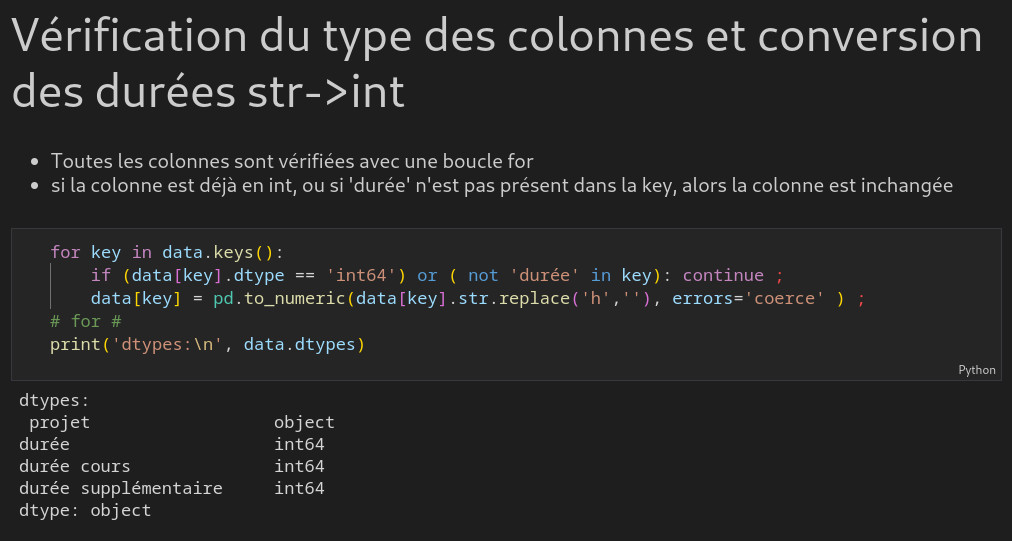
\includegraphics[width=110mm]{dates/cell-2.jpg}}%
	\only<3>{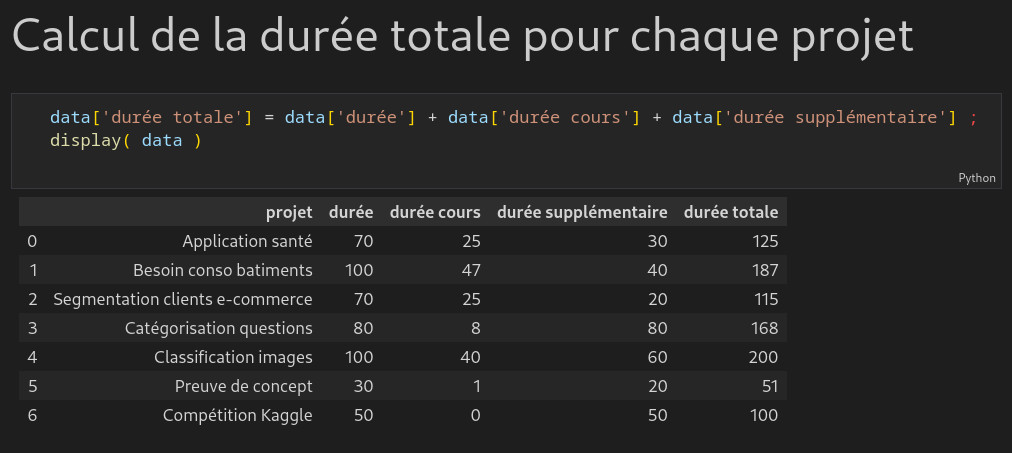
\includegraphics[width=110mm]{dates/cell-3.jpg}}%
	\only<4>{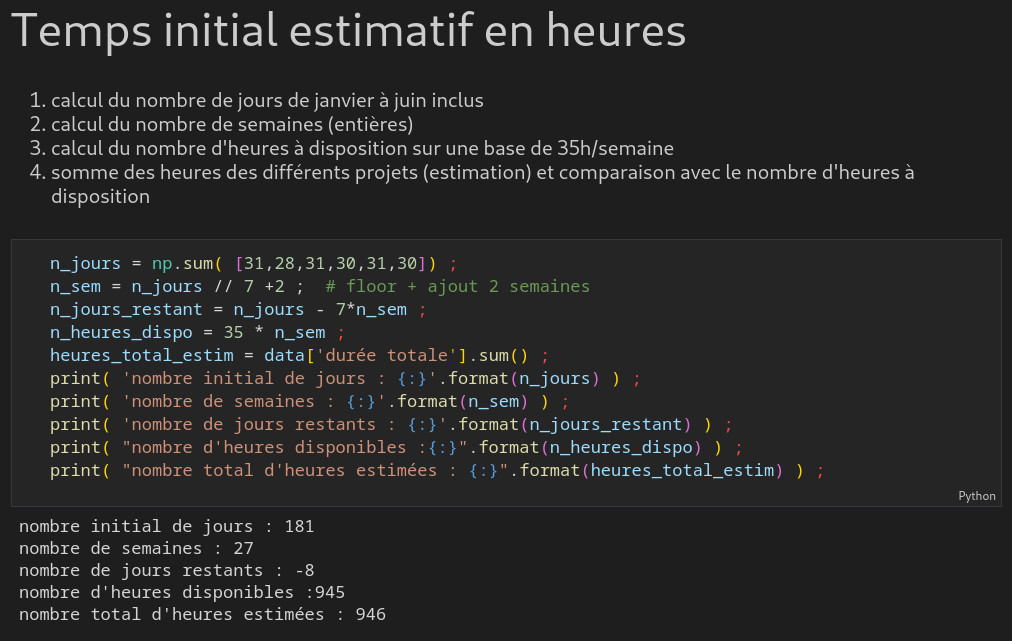
\includegraphics[width=110mm]{dates/cell-4.jpg}}%
	\only<5>{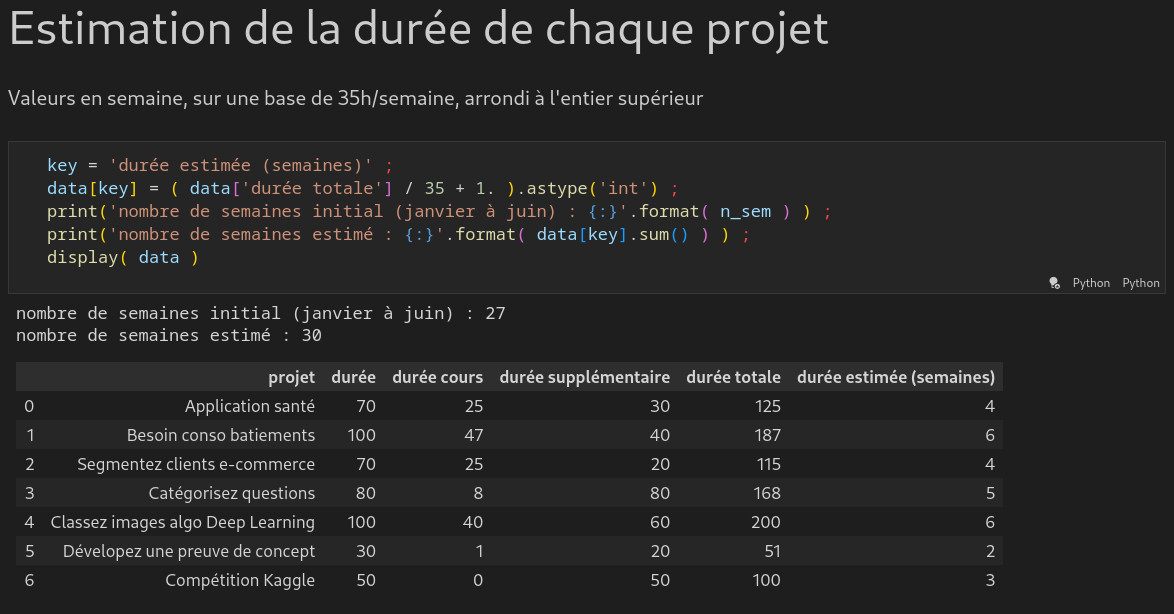
\includegraphics[width=110mm]{dates/cell-5.jpg}}%
	\only<6>{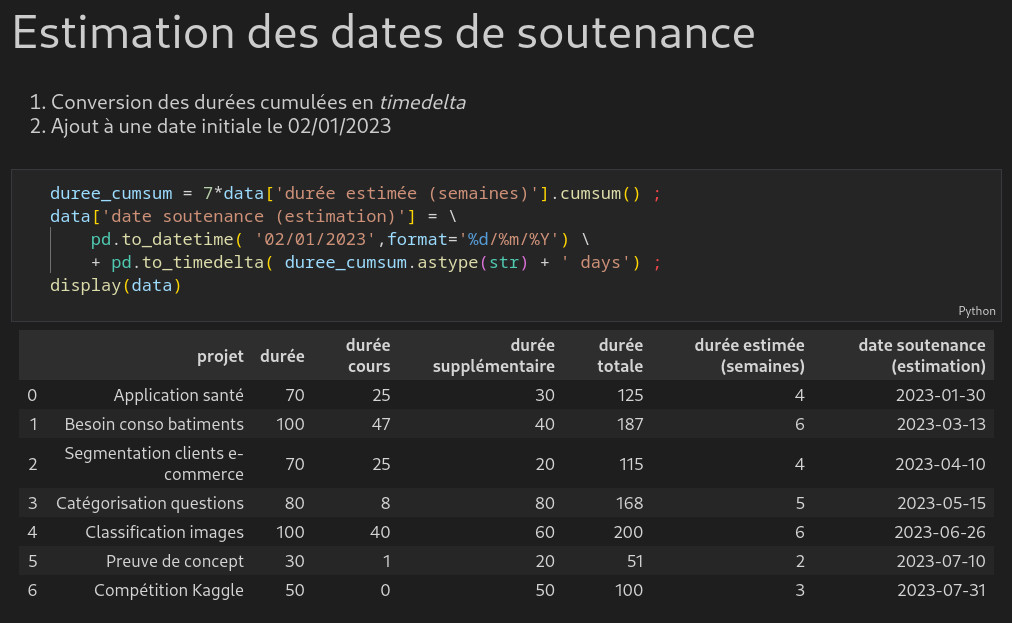
\includegraphics[width=110mm]{dates/cell-6.jpg}}%
	\only<7>{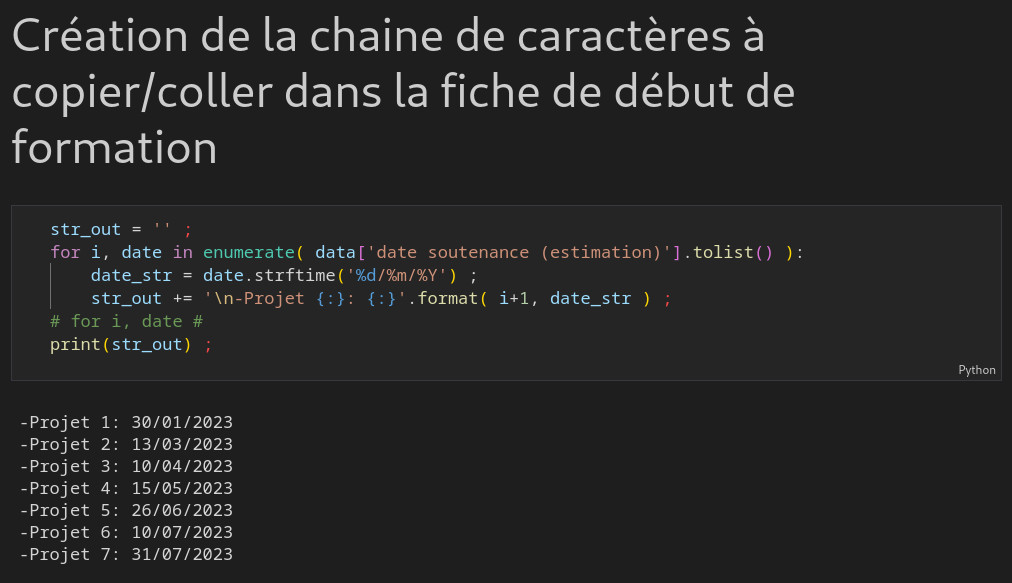
\includegraphics[width=110mm]{dates/cell-7.jpg}}%
	% \only<9>{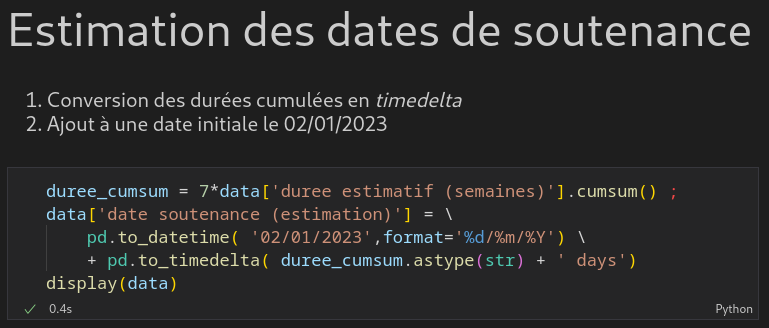
\includegraphics[width=110mm]{dates/cell-6.png}}%
	% \only<10>{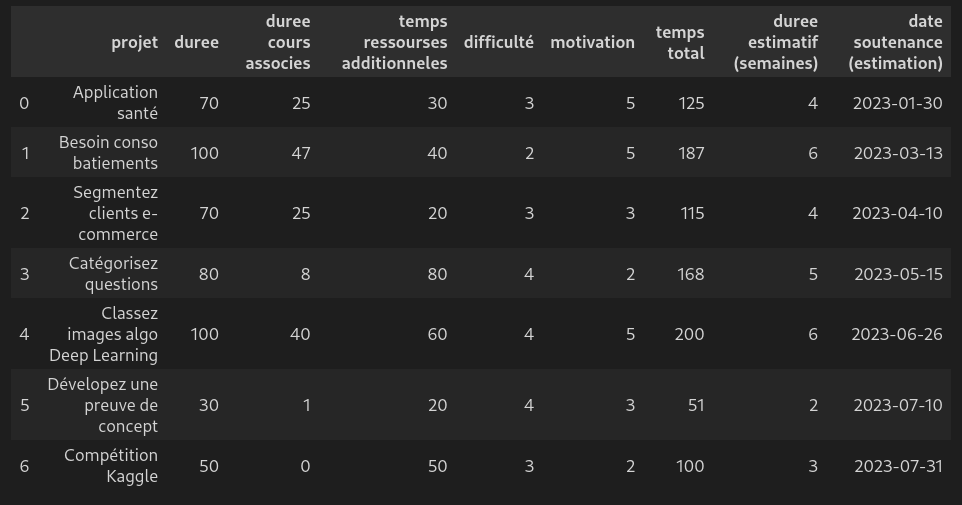
\includegraphics[width=110mm]{dates/cell-6_out.png}}%
	% \only<11>{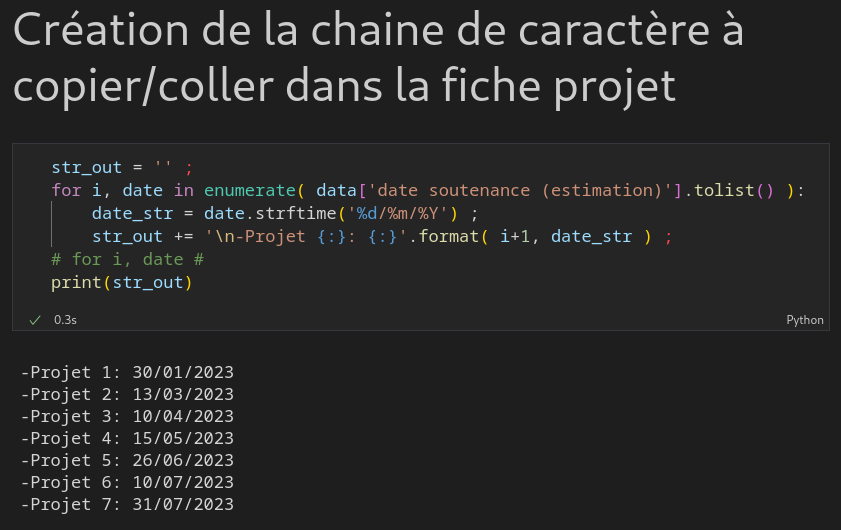
\includegraphics[width=110mm]{dates/cell-7.png}}%
	\vfill

\end{frame}

\section{Quelques bonnes pratiques}

\begin{frame}
	- Utiliser un calendrier et noter les date butoires de fin de projets
	- Utiliser la technique POMODORO (pour limiter la fatigue)
	- Bien préparer les sessions de mentorat, notamment en tenant à jour une liste de questions
	- Ne pas rester bloqué sur un point du projet en cours, avancer sur d'autres points non bloquants en attendant la prochaine session de mantorat / poser des questions à d'autres étudiants via la plateforme SLACK
\end{frame}




\section{Outils collaboratifs}

\begin{frame}
	- GitHub
	- Mails
	- Plateform OPENCLASSROOMS
	- Discord

	\only<1>{ \vspace*{0mm} 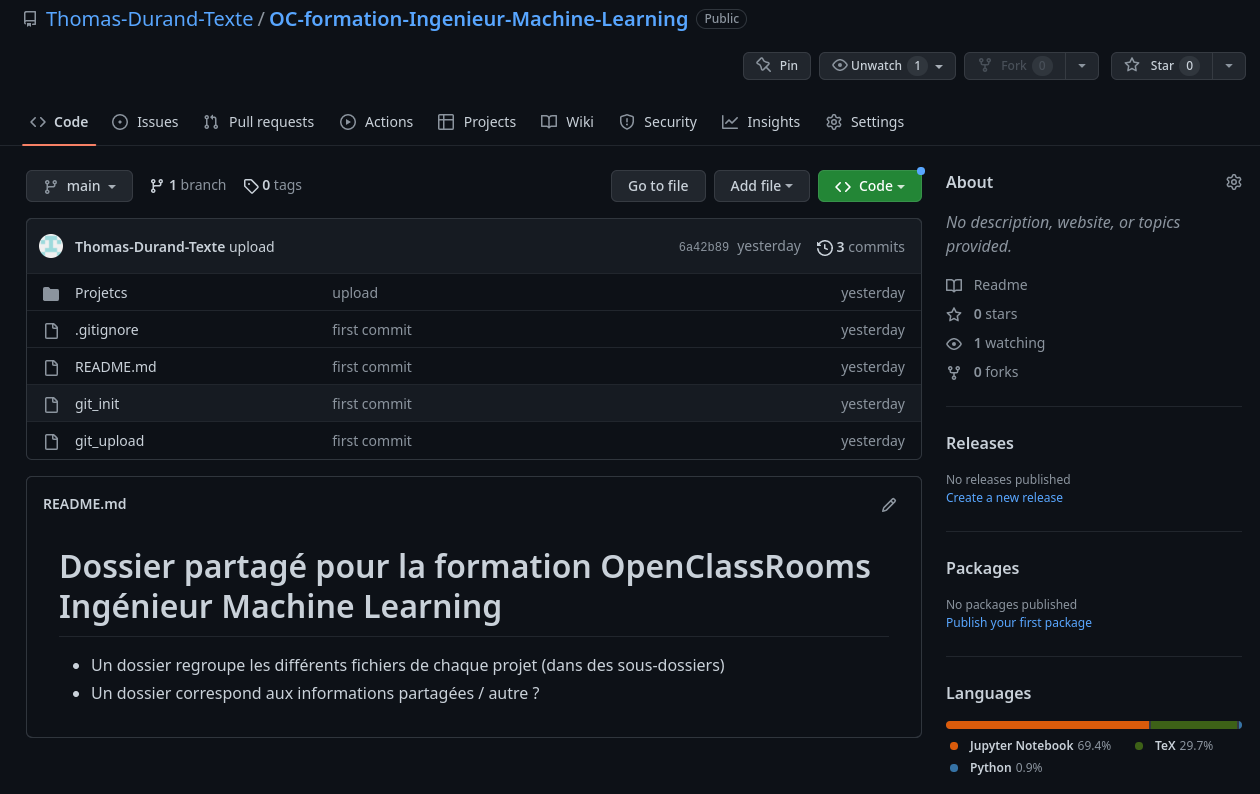
\includegraphics[width=100mm]{GitHub.png}}

\end{frame}




\begin{frame}[t]
	\vspace{18mm}
	\begin{center}
		\Large Merci pour votre attention.
	\end{center}

	\vfill
	{\tiny
	\begin{center}
		\alert{Artworks}\\ \vspace{-2mm}
		\alert{\rule{40mm}{0.1mm}}
	\end{center}

	commons.wikimedia : 
	\begin{itemize}
		\item[$\bullet$] Mass Spring System Resonance.gif by Guillermo Bossio 
	\end{itemize}
	openclipart.org : 
	\begin{itemize}
		\item[$\bullet$] loudspeaker by forestgreen
		\item[$\bullet$] Prismatic Cloud Gears 2, Abstract Brain Triangles Prismatic by GDJ
		\item[$\bullet$] Time Project by lbear
		\item[$\bullet$] Laptop Computer Icon by kael\_179
	\end{itemize}
	}

\end{frame}


% ------------------------------------------- %

\end{document}
